\documentclass{article}

\usepackage{tikz}
\usepackage{pgfplots}
\usepackage{physics}
\usepackage{amsmath}


\title{Just some ramblings}
\author{B.J. Spijkerman}

\begin{document}

\maketitle

\section{3-D waveguide analytical}
Starting with the Maxwell equations in a linearly polarizable material, where there is no charge or current:
\begin{align*}
  \nabla\cdot\vec{D}&=0,\\
  \nabla\cdot\vec{B}&=0,\\
  \nabla\times\vec{E}&=-\pdv[]{\vec{H}}{t},\\
  \nabla\times\vec{H}&=\varepsilon/c^2\pdv[]{\vec{E}}{t}.\\
\end{align*}
Now we take the curl of the third equation and use the first and second,
\begin{align*}
  \nabla\times\nabla\vec{E}&=\nabla\times\left(-\pdv[]{\vec{H}}{t}\right),\\
  \nabla\left(\frac{1}{\varepsilon}\nabla\cdot\vec{D}\right)-\nabla^2\vec{E}&=-\pdv[]{}{t}\nabla\times\vec{H},\\
  -\nabla^2\vec{E}&=-\varepsilon/c^2\pdv[2]{\vec{E}}{t},\\
  \nabla^2\vec{E}-\varepsilon/c^2\pdv[2]{\vec{E}}{t}&=0.
\end{align*}
We now assume the field to be propagating along the z-direction such that $\vec{E}(x,y,z;t)=\vec{E}(x,y)e^{-i(k_zz-\omega t)}$. Substituting this into the wave equation gives,
\begin{align*}
  \left[\nabla_{\perp}^2+\pdv[2]{}{z}-\varepsilon/c^2\pdv[2]{}{t}\right]\vec{E}(x,y)e^{-i(k_zz-\omega t)}&=0,\\
  \left[\nabla_{\perp}^2+(-ik_z)^2-\varepsilon\frac{(-i\omega)^2}{c^2}\right]\vec{E}(x,y)&=0,\\
  \left[\nabla_{\perp}^2+\varepsilon\left(\frac{\omega}{c}\right)^2-k_z\right]\vec{E}(x,y)&=0.
\end{align*}
Now taking we can look for the scalar function $\phi(x,y)$ by: $\vec{E}(x,y)=\vec{E}_0\phi(x,y)$ and realize that $\varepsilon\left(\omega/c\right)^2=n^2k_0^2=k^2=k_{\perp}+k_z$,
\begin{align*}
  \left[\nabla_{\perp}^2+k_{\perp}^2\right]\phi(x,y)=0.
\end{align*}
This is the transverse Helmholtz equation. We now consider the geometry of a cylindrical perfectly conducting waveguide of radius $R$,
\begin{equation*}
  \left[\frac{1}{r}\pdv[]{}{r}\left(r\pdv[]{}{r}\right)+\frac{1}{r^2}\pdv[2]{}{\theta}+k_{\perp}^2\right]\phi(r,\theta)=0,
\end{equation*}
We look for separable solutions of the kind $\phi(r,\theta)=R(r)\Theta(\theta)$,
\begin{align*}
  \frac{\Theta(\theta)}{r}\dv[]{}{r}\left(r\dv[]{R}{r}\right)+\frac{R(r)}{r^2}\dv[2]{\Theta}{\theta}+k_{\perp}^2R(r)\Theta(\theta)&=0,\\
  \frac{1}{rR(r)}\dv[]{}{r}\left(r\dv[]{R}{r}\right)+\frac{1}{r^2\Theta(\theta)}\dv[2]{\Theta}{\theta}+k_{\perp}^2&=0,\\
  \left[\frac{r^2}{R(r)}\dv[2]{R}{r}+\frac{r}{R(r)}\dv[]{R}{r}+(rk_{\perp})^2\right]+\left[\frac{1}{\Theta(\theta)}\dv[]{\Theta}{\theta}\right]&=0=\nu^2-\nu^2.
\end{align*}
We now use $\nu$ to separate the two equations,
\begin{align*}
  r^2\dv[2]{R}{r}+r\dv[]{R}{r}+\left(r^2k_{\perp}^2-\nu^2\right)R(r)&=0,\\
  \dv[2]{\Theta}{\theta}+\nu^2\Theta(\theta)&=0,
\end{align*}
where the second equation is solved by the integrating factor $i\nu\theta$. To solve the first equation we switch to the variable $y=k_{\perp}r$.
\begin{equation*}
  y^2\dv[2]{R}{y}+y\dv{R}{y}+\left(y-\nu^2\right)R(y),
\end{equation*}
this is Bessel's equation, solved by the Bessel function $J_\nu(k_{\perp}r)$. The total solution to the differential equation is then,
\begin{equation*}
  \phi(r,\theta)=R(r)\Theta(\theta)=J_\nu(k_{\perp}r)e^{i\nu\theta}.
\end{equation*}
The perfect conductor at $R$ from the origin implies the boundary condition $\phi(R,\theta)=J_\nu(k_{\perp}R)e^{i\nu\theta}=0$, which is equivalent to,
\begin{equation*}
  J_\nu(k_{\perp}R)=0,
\end{equation*}
we thus need to look for the zeros of the Bessel function, for $k_{\perp}R >> 1$ we can do this using the asymptotic approximation, which approximates the Bessel function far from the origin with a shifted cosine,
\begin{align*}
  J_\nu(k_{\perp}R)\approx\sqrt{\frac{2}{\pi k_{\perp}R}}\cos\left(k_{\perp}R-\frac{\nu\pi}{2}-\frac{\pi}{4}\right)&=0,\\
  k_{\perp}R-\frac{\nu\pi}{2}-\frac{\pi}{4}&=\frac{\pi}{2}+\pi n,\\
  k_{\perp,n}&=\frac{3+2\nu+4n}{4R}\pi.
\end{align*}
There is thus a set $\left\{k_{\perp,n}\right\}$ for each angular mode, implying the existence of a set $\left\{\phi_{\nu,n}(r,\theta)\right\}$. We can show this is an orthogonal basis by considering the inner product,
\begin{align*}
  \left<\phi_{\nu,n}\phi_{\mu,m}\right>&=\int_0^{2\pi}d\theta\int_0^{\infty}dr\,r\phi^*_{\nu,n}(r,\theta)\phi_{\nu,m}(r,\theta),\\
  &=\int_0^{2\pi}d\theta\int_0^{\infty}dr\,rJ_{\nu}(k_{\perp,n}r)e^{-i\nu\theta}J_{\mu}(k_{\perp,m}r)e^{i\mu\theta},\\
  &=\int_0^{2\pi}d\theta\,e^{i(\mu-\nu)\theta}\int_0^{\infty}dr\,rJ_{\nu}(k_{\perp,n}r)J_{\mu}(k_{\perp,m}r),\\
  &=\delta_{\nu,\mu}\int_0^{\infty}dr\,rJ_{\nu}(k_{\perp,n}r)J_{\nu}(k_{\perp,m}),\\
  &=\frac{1}{k_{\perp,n}}\delta\left(k_{\perp,n}-k_{\perp,m}\right)\delta_{\nu,\mu}
\end{align*}
The orthogonality of the functions $\phi_{\nu,n}$ implies that we in analogy with quantum mechanics can do a basis expansion,
\begin{equation*}
  \xi(r,\theta)=\bra{r,\theta}\ket{\xi}=\sum_{\nu,n}\bra{r,\theta}\ket{\phi_{\nu,n}}\bra{\phi_{\nu,n}}\ket{\xi}=\sum_{\nu,n}C_{\nu,n}\phi_{\nu,n}(r,\theta).
\end{equation*}
We can this calculate the constants $C_{\nu,n}$ as,
\begin{equation*}
  C_{\nu,n}=\int_0^{2\pi}d\theta\int_0^{\infty}dr\,r\phi_{\nu,\theta}^*(r,\theta)\xi(r,\theta),
\end{equation*}
we can continue by using Fourier transform to expand the $\xi$ in a series of rotationally symmetric functions $\xi(r,\theta)=\sum_{\nu}\xi_{\nu}(r)e^{i\nu\theta}$, with:
\begin{equation*}
  \xi_{\nu}=\frac{1}{\sqrt{2\pi}}\int_0^{2\pi}d\theta\, \xi(t,\theta)e^{i\nu\theta}.
\end{equation*}
When we now substitute this into the expression for $C_{\nu,n}$,
\begin{align*}
  C_{\nu,n}&=\int_0^{2\pi}d\theta\int_0^{\infty}dr\,rJ_{\nu}(k_{\perp,n}r)e^{-i\nu\theta}\sum_{\mu}\xi_{\mu}(r)e^{i\mu\theta},\\
  &=\sum_{\mu}\int_0^{\infty}d\theta\,e^{i(\mu-\nu)\theta}\int_0^{\infty}dr\,rJ_{\nu}(k_{\perp,n}r)\xi_{\mu}(r),\\
  &=\sum_{\mu}\delta_{\mu,\nu}\int_0^{\infty}dr\,rJ_{\nu}(k_{\perp,n}r)\xi_{\mu}(r),\\
  &=\int_0^{\infty}dr\,rJ_{\nu}(k_{\perp,n}r)\xi_{\nu}(r).
\end{align*}
This is the Hankel transformation. Now we apply this tho a Gaussian beam profile such that,
\begin{equation*}
  \xi(r)=\frac{\omega_0}{\omega(z)}\exp{-\left(r/\omega(z)\right)^2}.
\end{equation*}
Note that in this case $\nu=0$ we thus have only one constant to determine,
\begin{align*}
  C_{n}&=\int_0^{\infty}dr\,rJ_0(k_{\perp,n}r)\frac{\omega_0}{\omega(z)}\exp{-\left(r/\omega(z)\right)^2},\\
  &=\frac{\omega_0}{\omega(z)}\sum_{i=0}^{\infty}\frac{(-i)^i\left(\frac{k_{\perp,n}}{2}\right)^{2i}}{i!\Gamma(i+1)}\int_0^{\infty}dr\,r^{2i+1}\exp{-\left(r/\omega(z)\right)^2},\\
\end{align*}
We now transform the integration variable to $\chi=r/\omega(z)$,
\begin{align*}
  C_{n}&=\frac{\omega_0}{\omega(z)}\sum_{i=0}^{\infty}\frac{(-i)^i\left(\frac{k_{\perp,n}}{2}\right)^{2i}}{i!\Gamma(i+1)}\int_0^{\infty}d\chi\,\omega(z)\left[\chi\omega(z)\right]^{2i+1}\exp{-\chi^2},\\
  &=\omega_0\omega(z)\sum_{i=0}^{\infty}\frac{(-1)^i\left(\frac{k_{\perp,n}\omega(z)}{2}\right)^{2i}}{i!\Gamma(i+1)}\int_0^{\infty}d\chi\,\chi^{2i+1}\exp{-\chi^2}.
\end{align*}
We now transform to the variable $\eta=\chi^2$,
\begin{equation*}
  C_n=\omega_0\omega(z)\sum_{i=0}^{\infty}\frac{(-1)^i\left(\frac{k_{\perp}\omega(z)}{2}\right)^{2i}}{i!\Gamma(i+1)}\int_0^{\infty}d\eta\,\eta^{s-1}e^{-\eta},
\end{equation*}
where $s=i+1$, the integral is then the gamma function of $i+1$, such that,
\begin{align*}
  C_n&=\omega_0\omega(z)\sum_{i=0}^{\infty}\frac{(-1)^i\left(\frac{k_{\perp,n}\omega(z)}{2}\right)^{2i}\Gamma(i+1)}{i!\Gamma(i+1)},\\
  &=\omega_0\omega(z)\sum_{i=0}^{\infty}\frac{1}{i!}\left[-\left(\frac{k_{\perp,n}\omega(z)}{2}\right)^2\right]^i,\\
  &=\omega_0\omega(z)\exp{-\left(k_{\perp,n}\omega(z)/2\right)^2}.
\end{align*}
We can thus express a Gaussian beam profile as,
\begin{align*}
  \xi(r,\theta)&=\sum_{n=0}^{k_{\perp,\text{max}}}\omega_0\omega(z)\exp{-\left(k_{\perp,n}\omega(z)/2\right)^2}\phi_{0,n}(r,\theta),\\
  &=\omega_0\omega(z)\sum_{n=0}^{n_{\text{max}}}\exp{-\left(k_{\perp,n}\omega(z)/2\right)^2}J_{0}(k_{\perp,n}).
\end{align*}
So while the Gaussian beam cannot excite angular modes beyond zeroth order it has plenty of momentum states $\{k_{\perp,n}\}$ to explore. so then for the electromagnetic energy we get,
\begin{align*}
  E&\propto\left<|\vec{E}|^2\right>=\left<\xi^*_{\nu,n}(r,\theta)e^{-i\varphi(z)}\xi_{\mu,m}(r,\theta)e^{i\varphi(z)}\right>,\\
  &=\int_0^{\infty}d\theta\int_0^{\infty}dr\,r\sum_{\nu,n}C_{\nu,n}J_{\nu}(k_{\perp,n}r)e^{-i\theta}\sum_{\mu,m}C_{\mu,m}J_{\mu}(k_{\perp,m})e^{i\mu\theta},\\
  &=\sum_{\nu,\mu}\int_0^{\infty}d\theta\,e^{i(\mu-nu)\theta}\sum_{n,m}\int_0^{\infty}dr\,rJ_{\nu}(k_{\perp,n}r)J_{\mu}(k_{\perp,m}r)C_{\nu,n}C_{\mu,m},\\
  &=\sum_{\nu,\mu}\delta_{\mu,\nu}\sum_{n,m}\frac{1}{k_{\perp,n}}\delta(k_{\perp,n}-k_{\perp,m})C_{\nu,n}C_{\mu,m},\\
  &=\sum_{\nu,n}\frac{|C_{\nu,n}|^2}{k_{\perp,n}}=\sum_{\nu,n}\frac{4R|C_{\nu,n}|^2}{\pi(3+2\nu+4n)}.
\end{align*}
For the Gaussian beam profile discussed earlier we set $\nu=0$,
\begin{align*}
  E&\propto\sum_{n}\omega_0\omega(z)\exp{-\left(k_{\perp,n}\omega(z)\right)^2}\frac{1}{k_{\perp,n}},\\
  &=\omega_0\omega(z)\sum_{n}\exp{-\left(\frac{3+4n}{4R}\omega(z)\pi\right)^2}\frac{4R}{(3+4n)\pi},\\
  &=\frac{4R}{\pi}\omega_0\omega(z)\exp{-\left(\pi\omega(z)/4R\right)^2}\sum_{n}^{n_{\text{max}}}\frac{1}{3+4n}\exp{-\left(3+4n\right)^2}.
\end{align*}
To couple into a fiber we have to match the propagating wavevector,
\begin{equation*}
  k_z=\sqrt{\omega^2/c^2-k_{\perp,n}}=\sqrt{\frac{\omega^2}{c^2}-\left(\frac{(3+2\nu+4n)\pi}{4R}\right)^2},
\end{equation*}
for a propagating wave $Im\left[k_z\right]=0$ must hold which gives the constraint:
\begin{align*}
  \frac{\omega}{c}&>\frac{(3+2\nu+4n)\pi}{4R},\\
  \nu+2n&<2R\frac{\omega}{c}-\frac{3}{2},
\end{align*}
then when considering a Gaussian this is,
\begin{equation*}
  n<\frac{R\omega}{c}-\frac{3}{4}=Rk_0-\frac{3}{4}.
\end{equation*}

\newpage
We look at the interface of a 2D metal waveguide. Here the equation for the mode profiles perpendicular to the direction of propagation is.
\begin{equation*}
  \left[\pdv[2]{}{x}+k_x^2\right]\phi(x)=0.
\end{equation*}
The solutions to these equations are linear combinations of sines and cosines,
\begin{equation*}
  \phi(x)=A\sin(k_xx)+B\cos(k_xx),
\end{equation*}
the boundary conditions for a perfect conductor at $x=0\;\text{and}\;x=L$ is $phi(\pm L)=0$. This implies the coefficient $B$ to be zeros,
\begin{align*}
  \phi(L)&=\phi(L)=\sin(k_xL/2)=0.\\
  k_xL&=n\pi,\\
  k_x&=\frac{n\pi}{L}.
\end{align*}
This implies a set of wavevectors $\left\{k_{x,n}\right\}$. Now consider the inner product $\left<\phi_i\phi_j\right>$,
\begin{align*}
  \left<\phi_i\phi_j\right>&=\int_{-\infty}^{\infty}dx\,\left(\sin(k_{x,i}x)\right)^*\sin(k_{x,j}),\\
  &=\int_{-\infty}^{\infty}dx\,\left(e^{-ik_{x,i}x}-e^{ik_{x,i}x}\right)\left(e^{ik_{x,j}x}-e^{-ik_{x,j}x}\right),\\
  &=\int_{-\infty}^{\infty}dx\,\left(e^{i(k_{x,i}-k_{x,j})x}+e^{i(k_{x,j}-k_{x,i})x}-e^{-i(k_{x,i}+k_{x,j})x}+e^{i(k_{x,i}+k_{x,j})}\right),\\
  &=\int_{-\infty}^{\infty}dx\,\cos\left[(k_{x,i}-k_{x,j})x\right]+\sin\left[(k_{x,i}-k_{x,j})x\right]
\end{align*}
Does not seem to be an orthogonal basis. This SUCKS, it won't let me do the fun stuf. This leads me to the conclusion that the Ime thing is easier in 3D than in 2D, since in 3D we can use the expansion and sum to $n=R(z)k_{in}-\frac{3}{4}$. The overlap would remain essentially the same. Or what if I take the profile $\xi$ to be,
\begin{equation*}
  \xi(x)=\sum_{n=1}^{n_{\text{max}}}C_n\sin(k_{x,n}x),
\end{equation*}
where $C_n$ is then the Fourier transform of the function $\xi$, or lets start with,
\begin{align*}
  C&=\int_0^{L}dx\,
\end{align*}

\newpage
\section{FEM-waveguide 2-D}
To model the behaviour of a 2D waveguide the Finite Element Method (FEM) is used. The simplest case is to create a program to solve the homogenious Helmholtz equation in 2D. In this case we chose the waveguide to be a surface in the xy-plane with propogation of wave along the x-direction,
\begin{equation*}
  \left[\pdv[2]{}{y}+k_x\right]\phi(x,y)=0,
\end{equation*}
To to prevent reflection at the end of the domains we take the mirrors of the waveguide to be perfect conductors with Dirichlet boundary condition $\phi(x,0)=\phi(x,L_y)=0$. The inlet of the waveguide is excited with the analytical solution of the problem as to only excite $1$ mode. The end (outlet) of the waveguide is modeled with a round Robbin damping condition to prevent reflection back into the domain. This last point requires modifying the differential equation to,
\begin{equation*}
  \left[\pdv[2]{}{y}+k_y\right]\phi(x,y)=-\pdv[]{\phi}{x}\delta(x-L_x)=ik_x\phi(x,y)\delta(x-L_x),
\end{equation*}
to turn this into a variational problem we consider the inner product with some test function $\eta(x,y)$ with both sides of the equation,
\begin{equation*}
  \int_{\Omega}dxdy\,\left[\pdv[2]{\phi}{y}+k_y\phi\right]\eta=\int_{\partial\Omega}dy\,ik_x\phi\eta.
\end{equation*}
We use partial integration to make the left side more symmetric and end up with,
\begin{equation*}
  \int_{\Omega}dxdy\,\pdv[]{\phi}{y}\pdv[]{\eta}{y}+k_y\phi\eta-ik_x\int_{\partial\Omega}dy\,\phi\eta=0.
\end{equation*}
When excited with the mode,
\begin{equation*}
  f(x,y)=\sin(k_yy)e^{-ik_xx}.
\end{equation*}
We get the mode profile shown in Fig~\ref{fig:mode}.
\begin{figure}[!h]
  \centering
  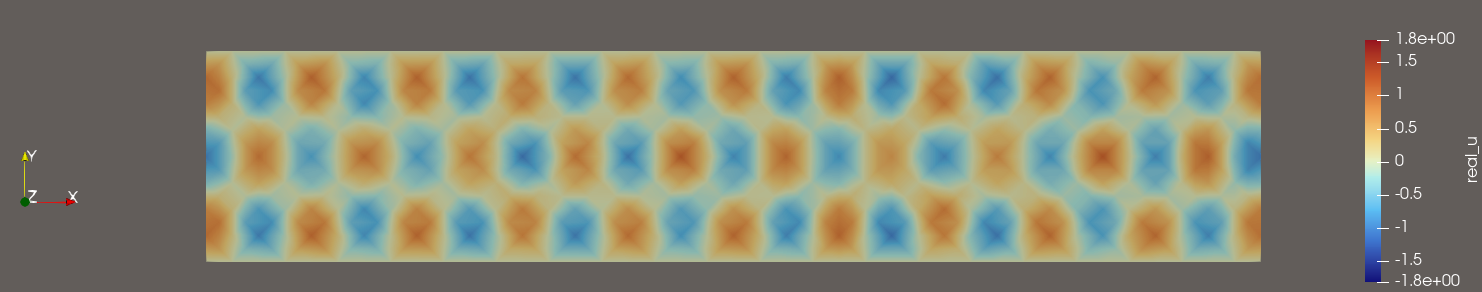
\includegraphics[width=\textwidth]{img/mode}
  \caption{Mode $n=3$.}
  \label{fig:mode}
\end{figure}

To turn this into a propagation problem we switch to the wave equation under the same boundary conditions,
\begin{equation*}
  \left[\nabla^2-\frac{}{c}\pdv[3]{}{t}\right]\phi(x,y,t)=-\pdv[2]{\phi}{x}\delta(x-L_x).
\end{equation*}
The variational form of this is similar to the previous equation,
\begin{align*}
  \int_{\Omega}dxdy\,\left[\nabla^2\phi-\frac{1}{c^2}\pdv[2]{\phi}{t}\right]\eta(x,y,t)&=-\int_{\partial\Omega}dy\,\pdv[]{\phi}{x}\eta(x,y,t),\\
  \int_{\Omega}dxdy\,\left(\nabla\phi\right)\cdot\left(\nabla\eta\right)+\frac{1}{c^2}\pdv[2]{\phi}{t}\eta&=\int_{\partial\Omega}dy\,\pdv[]{\phi}{x}\eta.
\end{align*}
We approximate the time derivative with the Euler scheme. In this we write down the recursive formula,
\begin{align*}
  \int_{\partial\Omega}dy\,\pdv[]{\phi}{x}\eta&=\int_{\Omega}dxdy\,\left(\nabla\phi\right)\cdot\left(\nabla\eta\right)+\frac{1}{c^2}\frac{\phi^{i+1}-2\phi^{i}+\phi^{i-1}}{\left(\Delta t\right)^2}\eta,\\
  \phi^{i+1}&=\int_{\Omega}dxdy\,\left(2\phi^i-\phi^{i-1}\right)\eta-\left(\Delta tc\right)^2\left(\nabla\phi\right)\cdot\left(\nabla\eta\right)+\left(\Delta tc\right)^2\int_{\partial\Omega}dy\,\pdv[]{\phi}{x}\eta
\end{align*}
To solve the system then we solve the spatial components of the problem using FEM and then explicitly time step using the forward Euler algorithm.
\end{document}


